

\begin{frame}[ctb!]
  \frametitle{Heat Limits In Geology}
  % table?
  Important heat limits in materials of the repository restrict loading designs 
  and capacity.
   \begin{table}[h!]
    \centering
    \footnotesize{
    \begin{tabularx}{\textwidth}{|X|c|c|X|}
      \multicolumn{4}{c}{\textbf{Models of Heat Load for Various Geologic Media}}\\
      \hline
      Source & Nation & Geology & Methodology \\  
      (Who) & (Where) & (What) & (How) \\  
      \hline
      Enresa \cite{von_lensa_red-impact_2008}           & Spain       & Granite       &  CODE\_BRIGHT 3D Finite Element \\ 
      NRI   \cite{von_lensa_red-impact_2008}            & Czech Rep.  & Granite       &  Specific Temperature Integral   \\
      ANDRA \cite{andra_granite:_2005}                  & France      & Granite       &  3D Finite Element CGM code   \\
      SKB \cite{ab_long-term_2006}                      & Sweden      & metagranite   &  1D-3D Site  Descriptive Models \\
      SCK$\cdot$CEN   \cite{von_lensa_red-impact_2008}  & Belgium     & Clay          &  Specific Temperature Integral   \\ 
      ANDRA \cite{andra_argile:_2005}                   & France      & Argile Clay   &  3D Finite Element CGM code   \\
      NAGRA \cite{johnson_project_2002, johnson_calculations_2002}  & Switzerland  & Opalinus Clay &  3D Finite Element CGM code \\
      GRS \cite{von_lensa_red-impact_2008}              & Germany     & Salt          &  HEATING (3D finite difference)   \\ 
      NCSU(Li)   \cite{li_examining_2007}               & USA         & Yucca Tuff    &  Specific Temperature Integral \\        
      NCSU(Nicholson) \cite{nicholson_thermal_2007}     & USA         & Yucca Tuff    &  COSMOL 3D Finite Element\\
      Radel \& Wilson \cite{radel_repository_2007}      & USA         & Yucca Tuff    &  Specific Temperature Change \\ 
      \hline
    \end{tabularx}
    \caption[International heat transport modeling methods in various geologic host media.]{Methods by which to calculate heat 
    load are independent of geology. Maximum heat load constraints, however, vary among host formations. }
    \label{tab:heat}
    }
  \end{table}

\end{frame}

% heat based capacity 
\begin{frame}[ctb!]
  \frametitle{Impact of Repository Designs}
  % lines, points, infinite lines, footprints.
   \begin{table}[h!]
  \centering
      \footnotesize{
      \begin{tabular}{|l|c|c|r|}
          \multicolumn{4}{c}{\textbf{Yucca Mounting Footprint Expansion Calculations}}\\
          \hline
          Author&Max. Capacity&Footprint&Details\\
          &$tonnes$&$km^2$&\\
          \hline
          &&&\\
          OCRWM&$70,000$&$4.65$&``statutory case''\\
          &$97,000$&$6$&``full inventory case''\\
          &$119,000$&$~7$&``additional case''\\
          \hline
          &&&\\
          Yim, M.S.&$75,187$&$4.6$&SRTA code\\
          &$76,493$&$4.6$&STI method\\
          &$95,970$&$4.6$&$63$m drift spacing\\
          &$82,110$&$4.6$&75 yrs. cooling\\
          \hline
          &&&\\
          Nicholson, M.&$103,600$&$4.6$&drift spacing\\
          \hline
          &&&\\
          EPRI&&&\\
          &$63,000$&$6.5$&Base Case CSNF\\
          option 1&$126,000$&$13$&expanded footprint\\
          option 2&$189,000$&$6.5$&multi-level design\\
          option 3&$189,000$&$6.5$&grouped drifts\\
          options 2+3&$252,000$&$6.5$&hybrid\\
          options 1+(2or3) &$378,000$&$13$&hybrid\\
          options 1+2+3 &$567,000$&$13$&hybrid\\
          \hline
        \end{tabular}
        \caption[Yucca Mountain Footprint Expansion Calculations]{Various analyses based on heat 
        load limited repository designs have resulted in footprint expansion calculations of the 
        YMR.} 
        \label{tab:footprint}
        }
      \end{table}

   \begin{figure}[h!]
     \begin{center}
       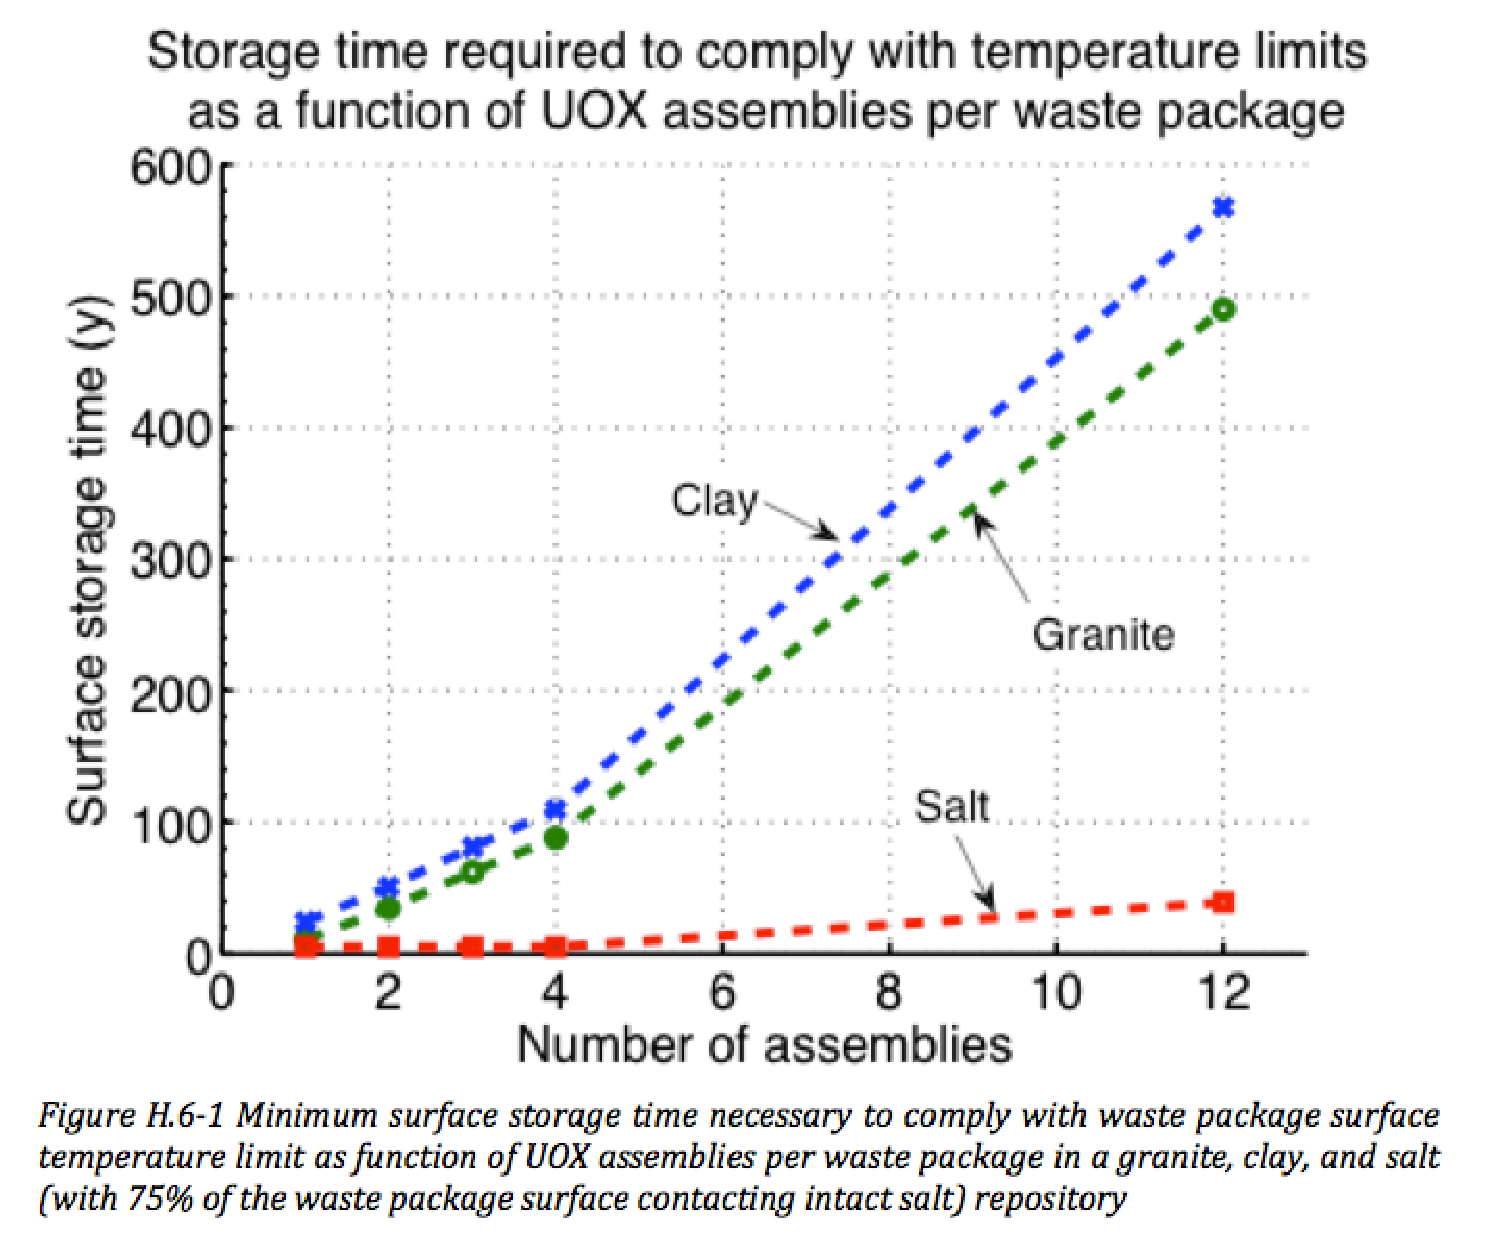
\includegraphics[height=.5\textheight]{./images/llnlGeos.eps}
     \end{center}
     \caption{LLNL has found that the higher heat limit, alcove geometry, and 
     high conductivity in salt allows for earlier loading times.}
     \label{fig:llnlGeos}
   \end{figure}
\end{frame}

% heat based capacity 
\begin{frame}[ctb!]
  \frametitle{Heat Based Capacity}
  % lines, points, infinite lines, footprints.
  \begin{minipage}{0.49\textwidth}
    \begin{figure}[h!]
        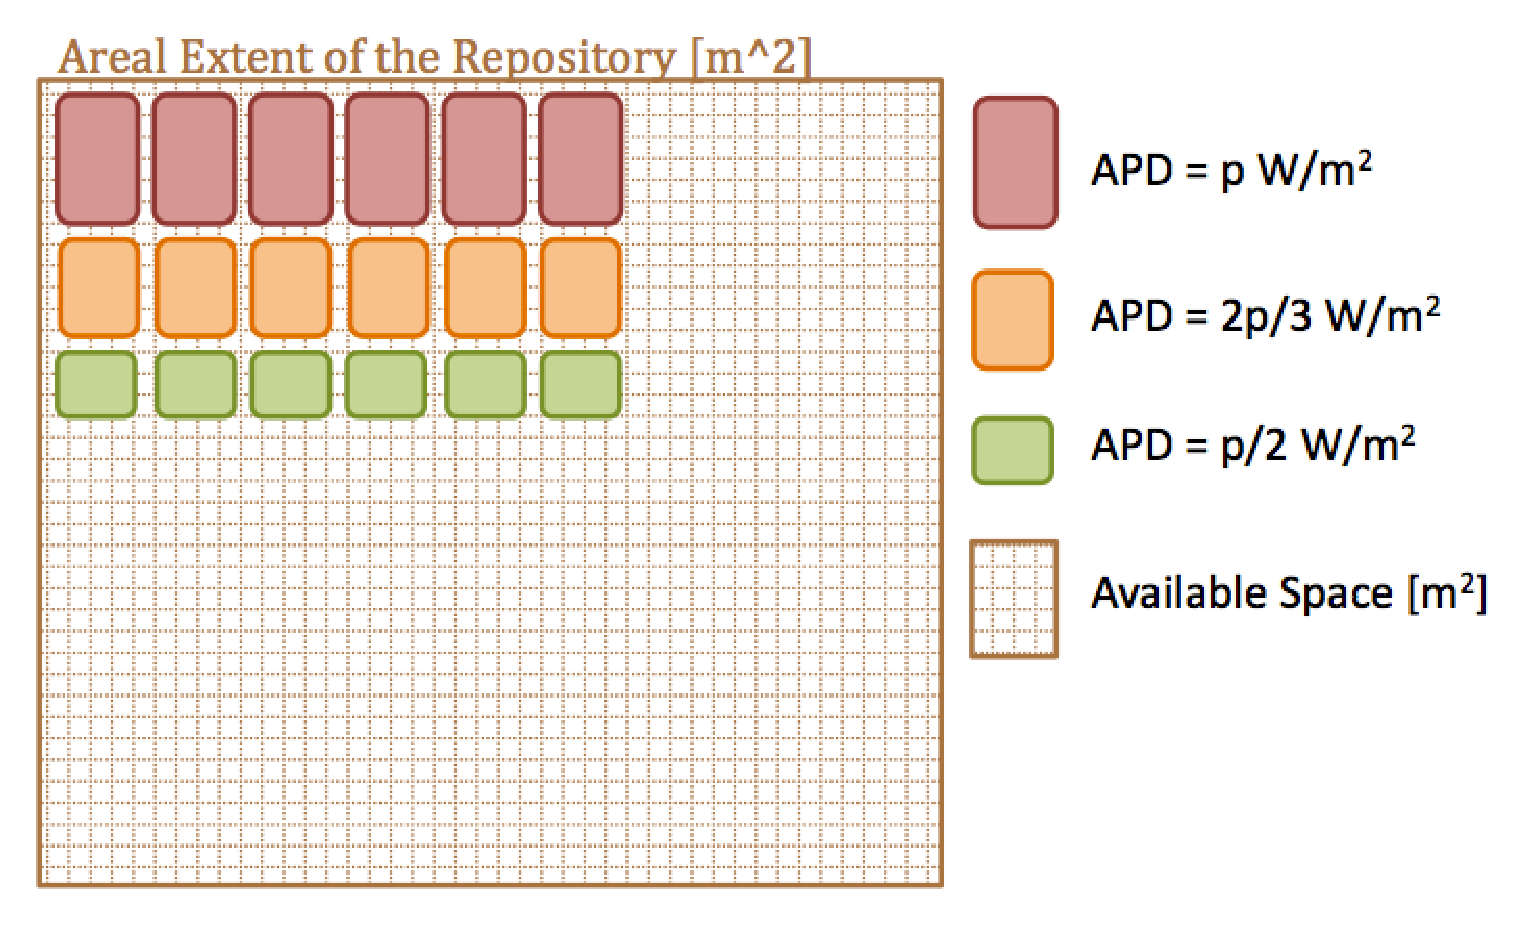
\includegraphics[width=0.9\textwidth]{./images/APD.eps}
      \caption{Areal Power Density (APD) can be used to determine appropriate 
      repository loading for arbitrary waste streams. }
      \label{fig:apd}
  \end{figure}
  \end{minipage}
  \hspace{0.01cm}
  \begin{minipage}{0.49\textwidth}
    Loading is subject to the constraints,
    \footnotesize{
    \begin{align}
      P_{tot} &\le P_{max} \\
      APD_i &\le APD_{max}
      \intertext{where}
      P_{max} &= A\cdot APD_{max}\\ 
      P_{tot} &= \sum_{i=0}^{N}n_i P_i\\ 
      P_i &= \mbox{power of package i}\nonumber\\
      n_i &= \mbox{ith package}\nonumber\\
      N &= \mbox{number of packages}\nonumber\\
      APD_{max} &= \mbox{max areal power density}\nonumber
    \end{align}
    }
  \end{minipage}
\end{frame}

\begin{frame}[ctb!]
  \frametitle{Detailed Techniques}
  % 2d,3d,finite diffs, etc.
   \begin{table}[h!]
    \centering
    \footnotesize{
    \begin{tabular}{|l|c|c|l|}
      \multicolumn{4}{c}{\textbf{Models of Heat Load for Various Geologies}}\\
      \hline
      Source & Nation & Geology & Methodology \\  
      (Who) & (Where) & (What) & (How) \\  
      \hline
      Enresa \cite{von_lensa_red-impact_2008}           & Spain       & Granite       &  CODE\_BRIGHT 3D Finite Element \\ 
      NRI   \cite{von_lensa_red-impact_2008}            & Czech Rep.  & Granite       &  Specific Temperature Integral   \\
      ANDRA \cite{andra_granite:_2005}                  & France      & Granite       &  3D Finite Element CGM code   \\
      SKB \cite{ab_long-term_2006}                      & Sweden      & metagranite   &  1D-3D Site  Descriptive Models \\
      SCK$\cdot$CEN   \cite{von_lensa_red-impact_2008}  & Belgium     & Clay          &  Specific Temperature Integral   \\ 
      ANDRA \cite{andra_argile:_2005}                   & France      & Argile Clay   &  3D Finite Element CGM code   \\
      NAGRA \cite{johnson_project_2002, johnson_calculations_2002}  & Switzerland  & Opalinus Clay &  3D Finite Element CGM code \\
      GRS \cite{von_lensa_red-impact_2008}              & Germany     & Salt          &  HEATING (3D finite difference)   \\ 
      NCSU(Li)   \cite{li_examining_2007}               & USA         & Yucca Tuff    &  Specific Temperature Integral \\        
      NCSU(Nicholson) \cite{nicholson_thermal_2007}     & USA         & Yucca Tuff    &  COSMOL 3D Finite Element\\
      Radel \& Wilson \cite{radel_repository_2007}      & USA         & Yucca Tuff    &  Specific Temperature Change \\ 
      \hline
    \end{tabular}
    \caption[Models for Heat Transport for Various Geologies]{Methods by which to calculate heat 
    load are independent of geology. Maximum heat load constraints, however, vary among host formations. }
    \label{tab:heat}
    }
  \end{table}

  Similar heat transport models can be used for all geologies, but are 
  differentiated by material parameters $(c_p, K, \rho)$ and different 
  thermal constraints.
\end{frame}


% SINDA 

\begin{frame}
  \frametitle{ANL model}
  A model created by the UFD team at Argonne national lab using the 
  SINDA{\textbackslash}G heat transport framework employs a lumped parameter 
  model and an optimization loop to arrive at a minimal drift spacing for a 
  given waste stream in agreement with user input thermal limits. 
  \begin{figure}[h!]
    \begin{center}
      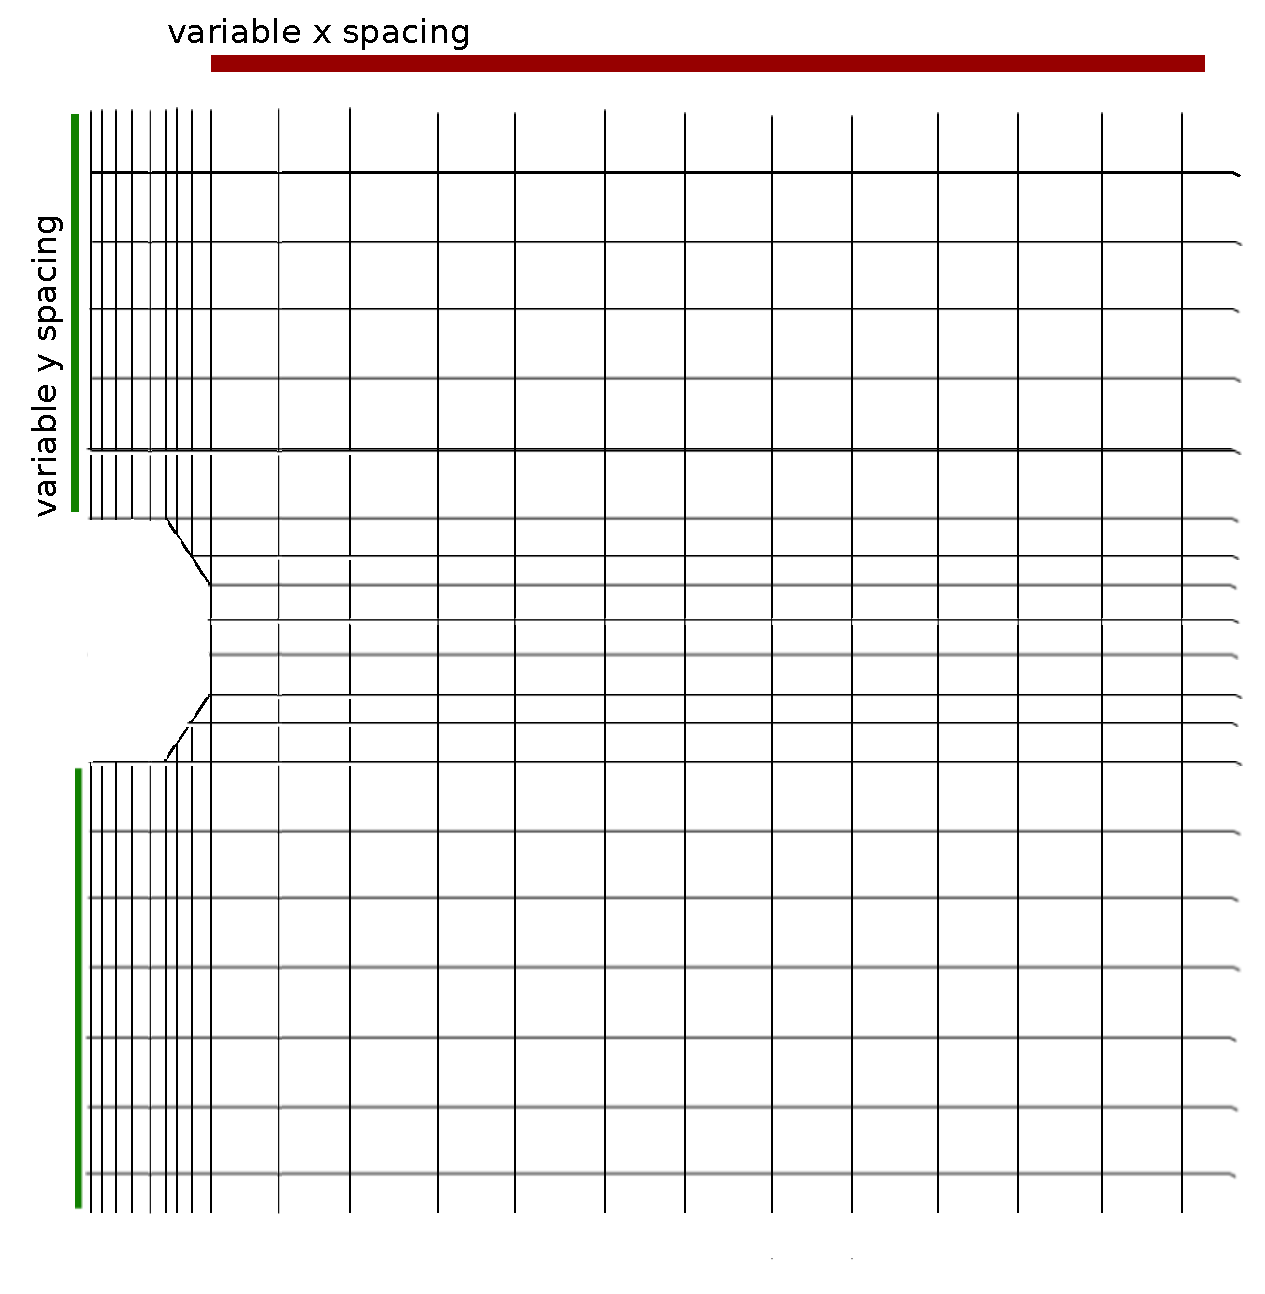
\includegraphics[height=.5\textheight]{../report/litrev/sindageom.eps}
    \end{center}
    \caption{Two adjustable geometric dimensions of the ANL model.} 
    \label{fig:sindageom}
  \end{figure}
\end{frame}


\begin{frame}[ctb!]
  \frametitle{Lumped Parameter Technique}
  % resistor diagram
  \begin{figure}[h!]
    \begin{center}
      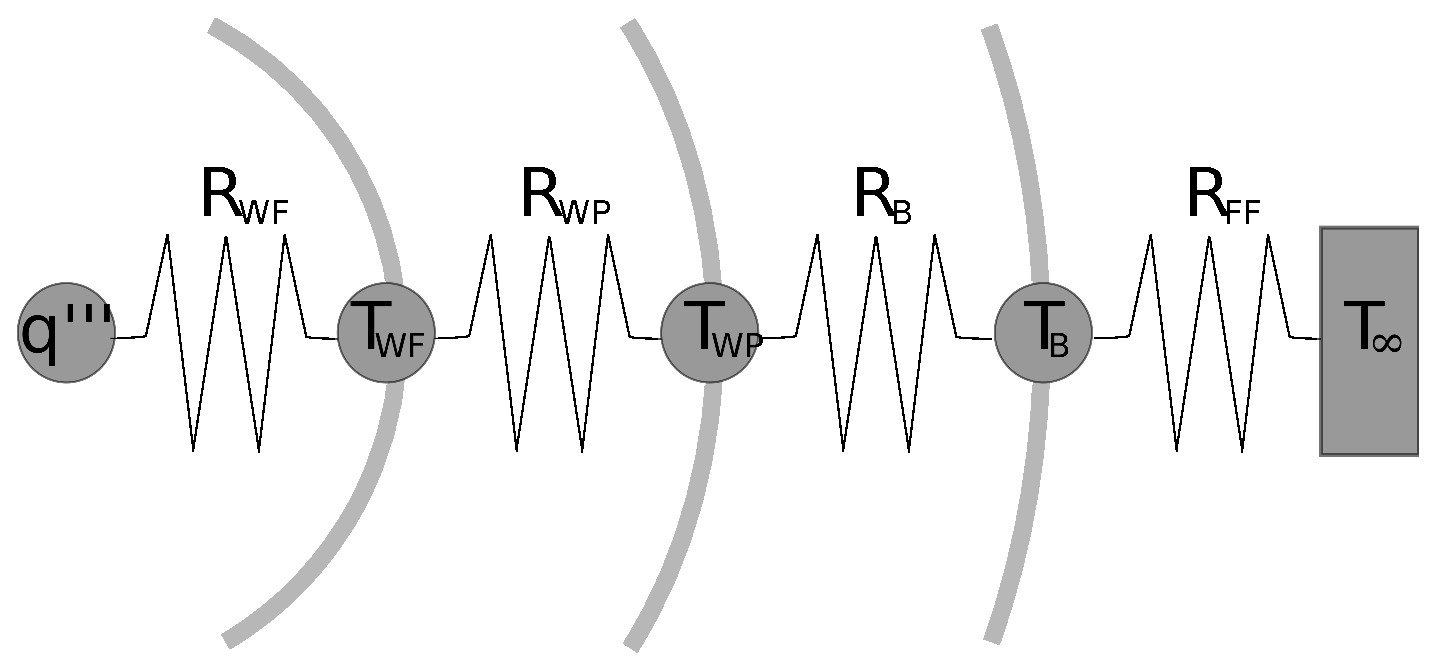
\includegraphics[width=0.9\textwidth]{./images/lumpedParam.eps}
    \end{center}
    \caption{The lumped parameter analogy used for heat transfer can be applied 
    as a one dimensional approximation to the disposal system concept. }
    \label{fig:lumpedParam}
  \end{figure}
\end{frame}


% LLNL

\begin{frame}
  \frametitle{LLNL Model : Geometry}
  \begin{minipage}{0.3\textwidth}
    \begin{figure}[h!]
      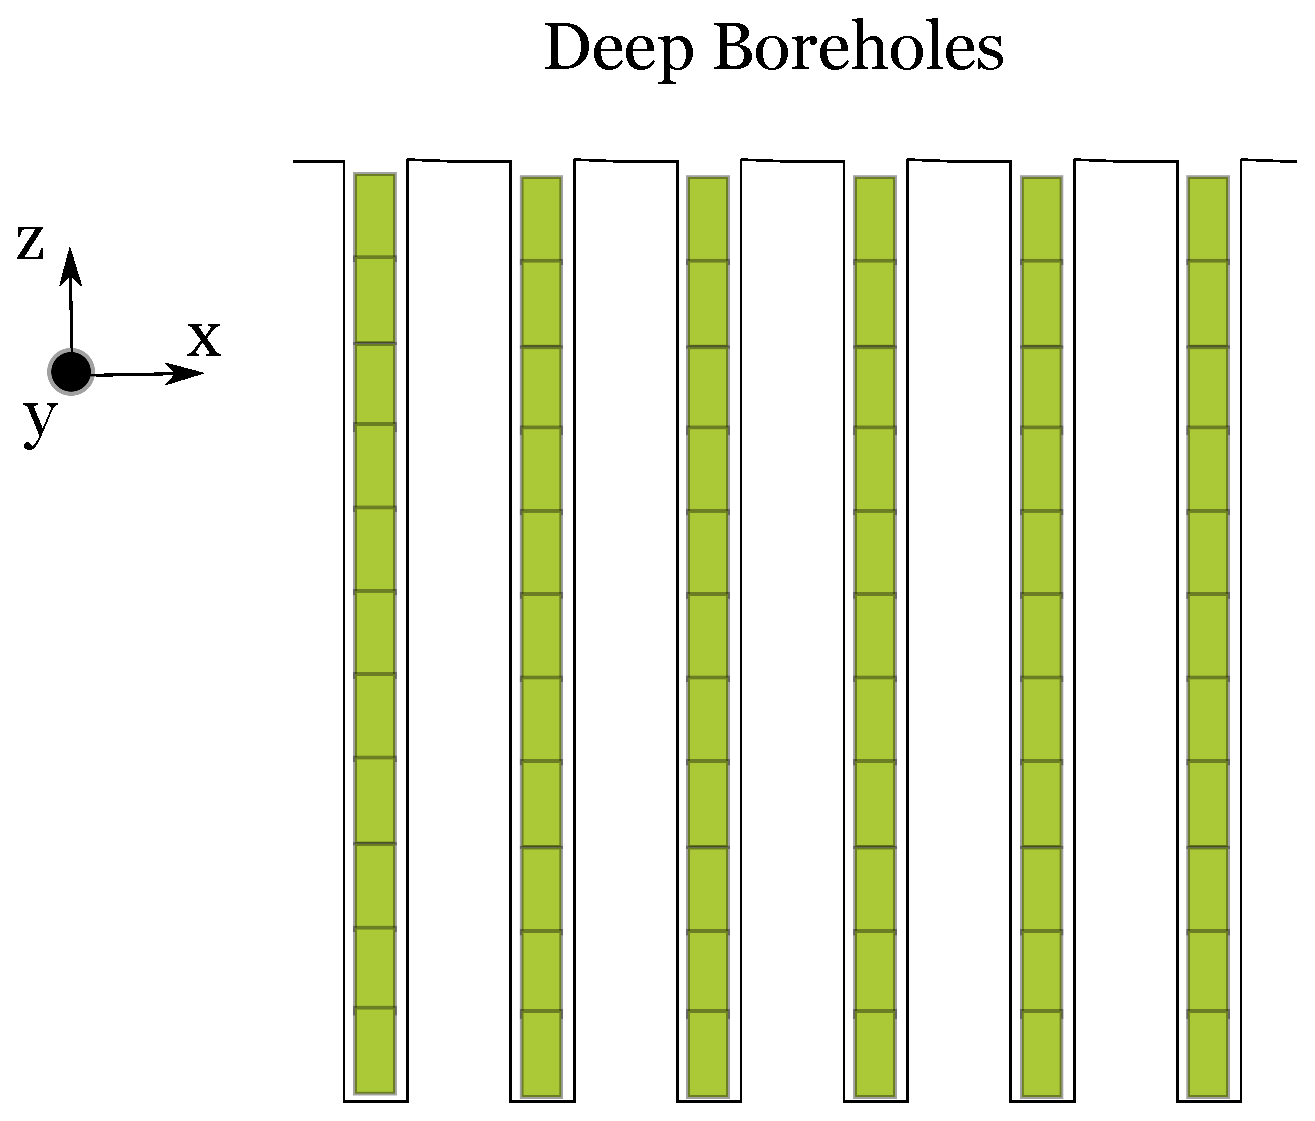
\includegraphics[width=\textwidth]{./images/boreholes.eps}
    \end{figure}
    \begin{figure}[h!]
      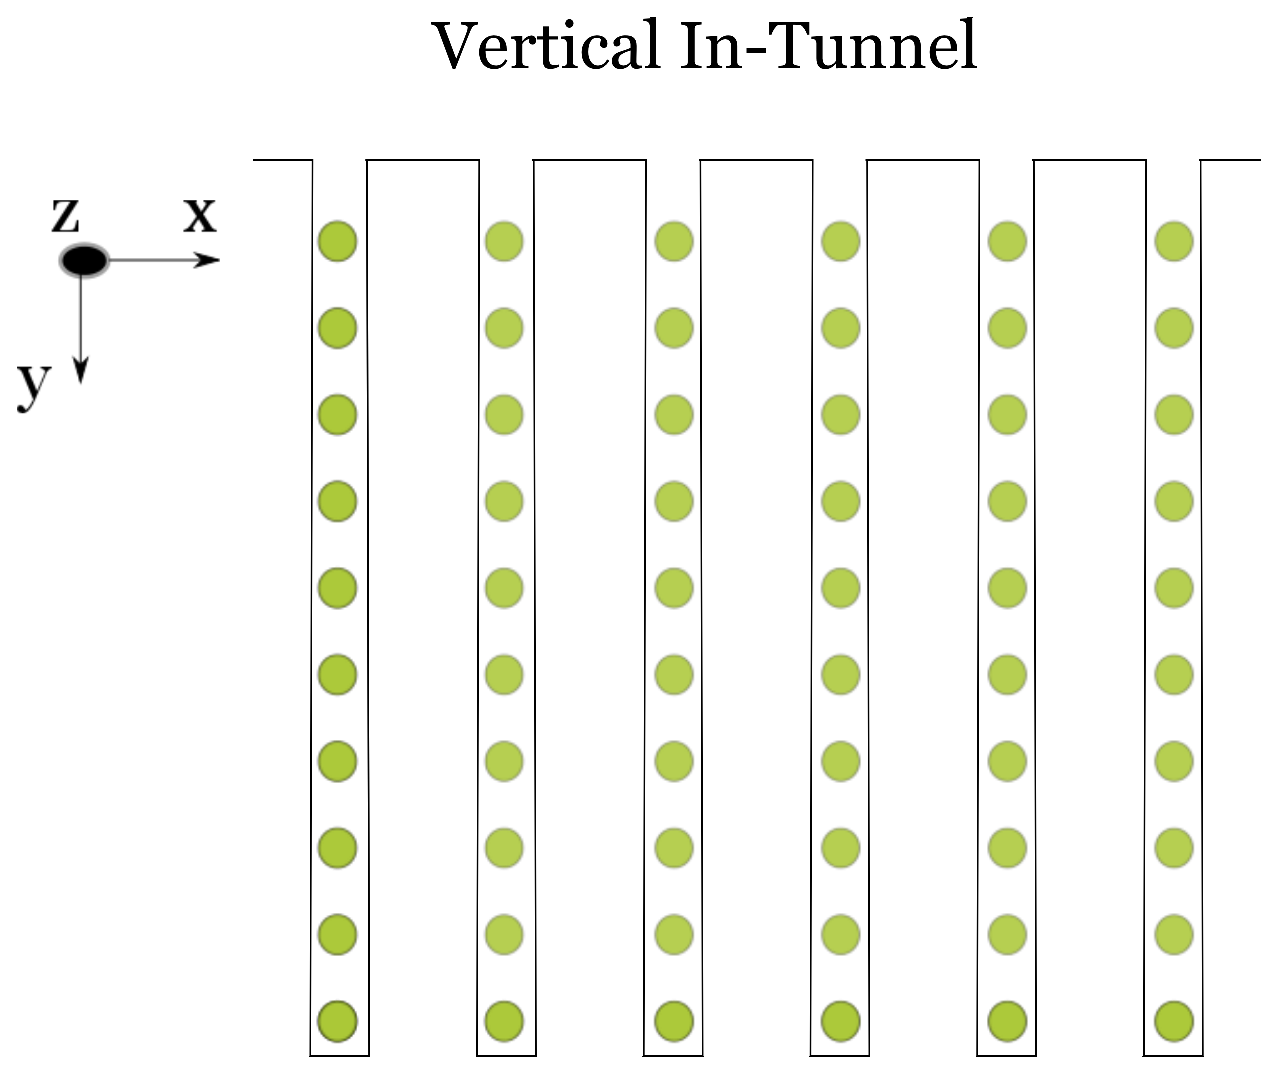
\includegraphics[width=\textwidth]{./images/vertical.eps}
    \end{figure}
  \end{minipage}
  \hspace{0.01cm}
  \begin{minipage}{0.3\textwidth}
    \begin{figure}[h!]
      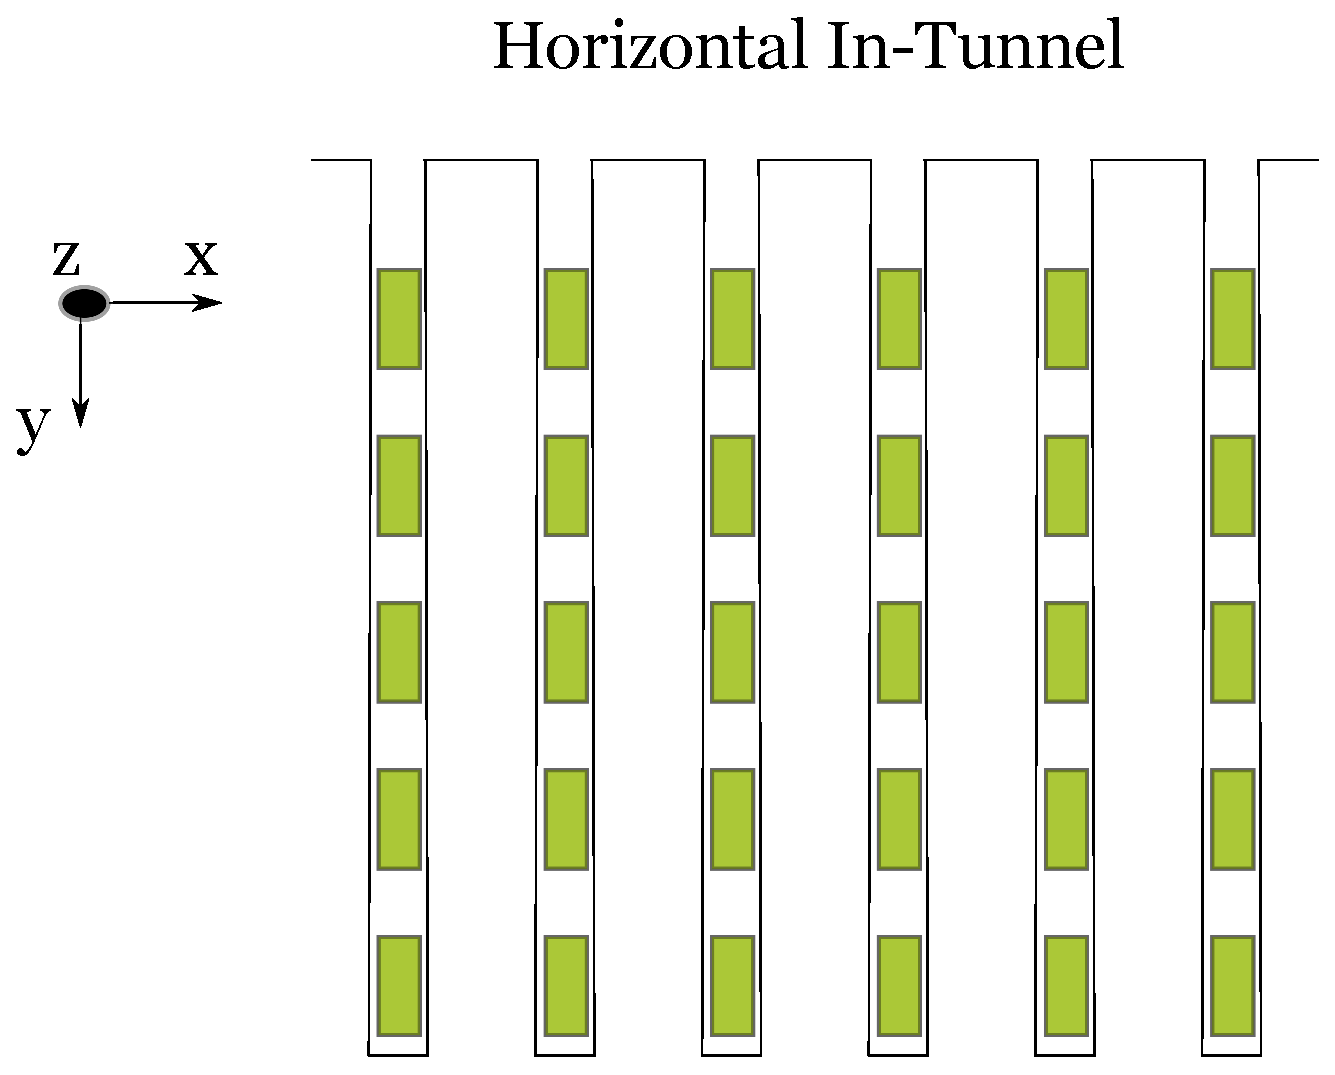
\includegraphics[width=\textwidth]{./images/horizontal.eps}
    \end{figure}
    \begin{figure}[h!]
      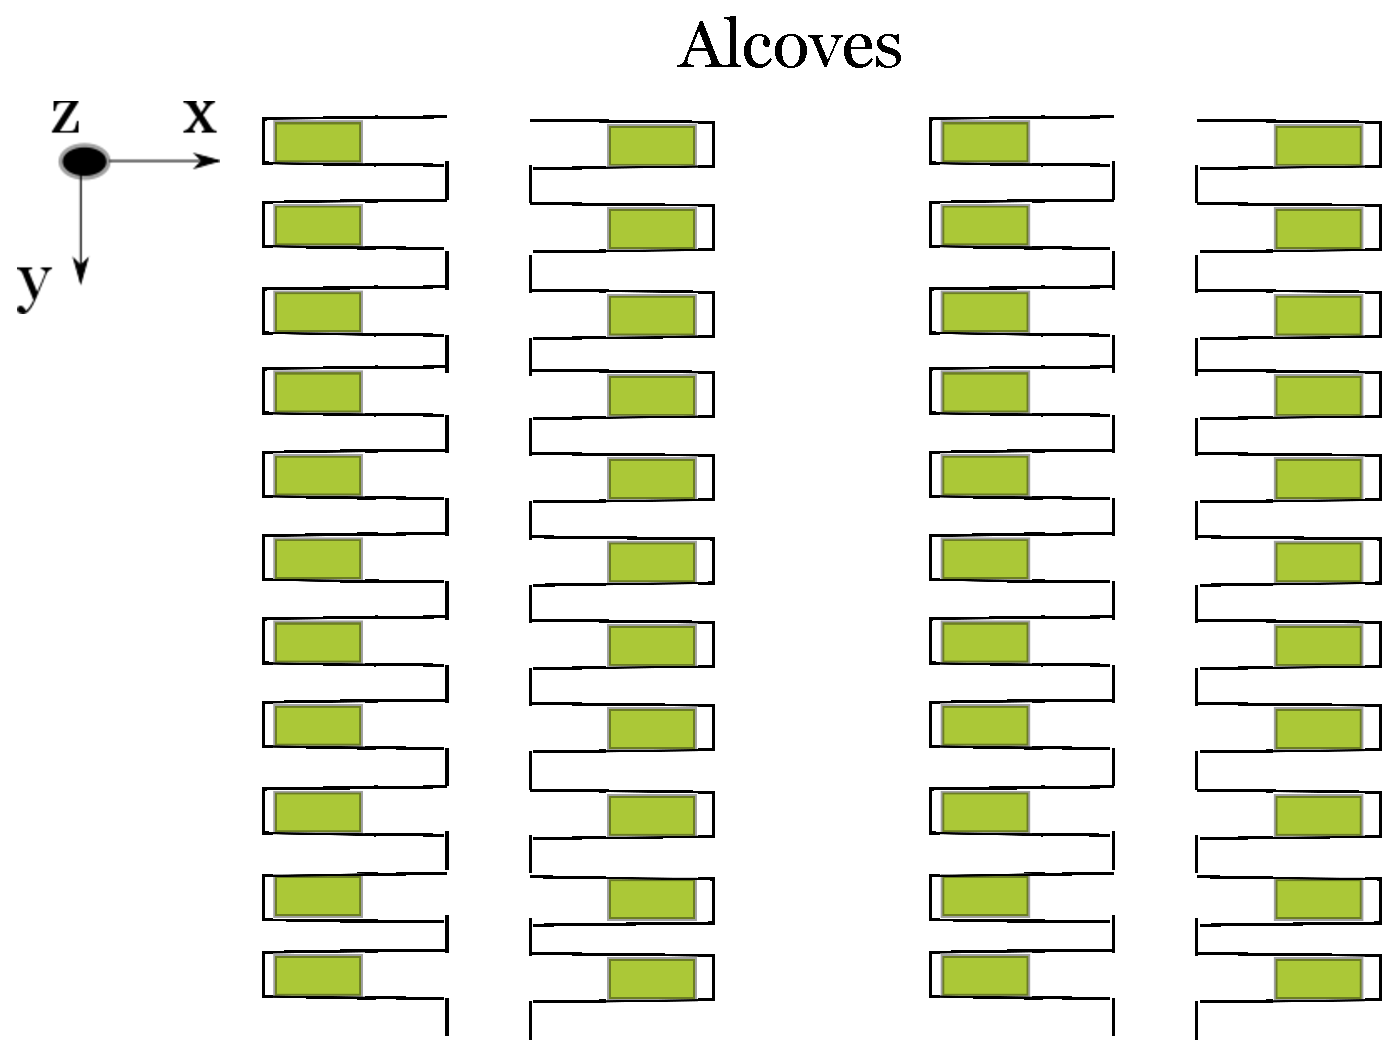
\includegraphics[width=\textwidth]{./images/alcoves.eps}
    \end{figure}
  \end{minipage}
  \hspace{0.01cm}\large{$=$}\hspace{0.01cm}
  \begin{minipage}{0.3\textwidth}
    \begin{figure}[b]
      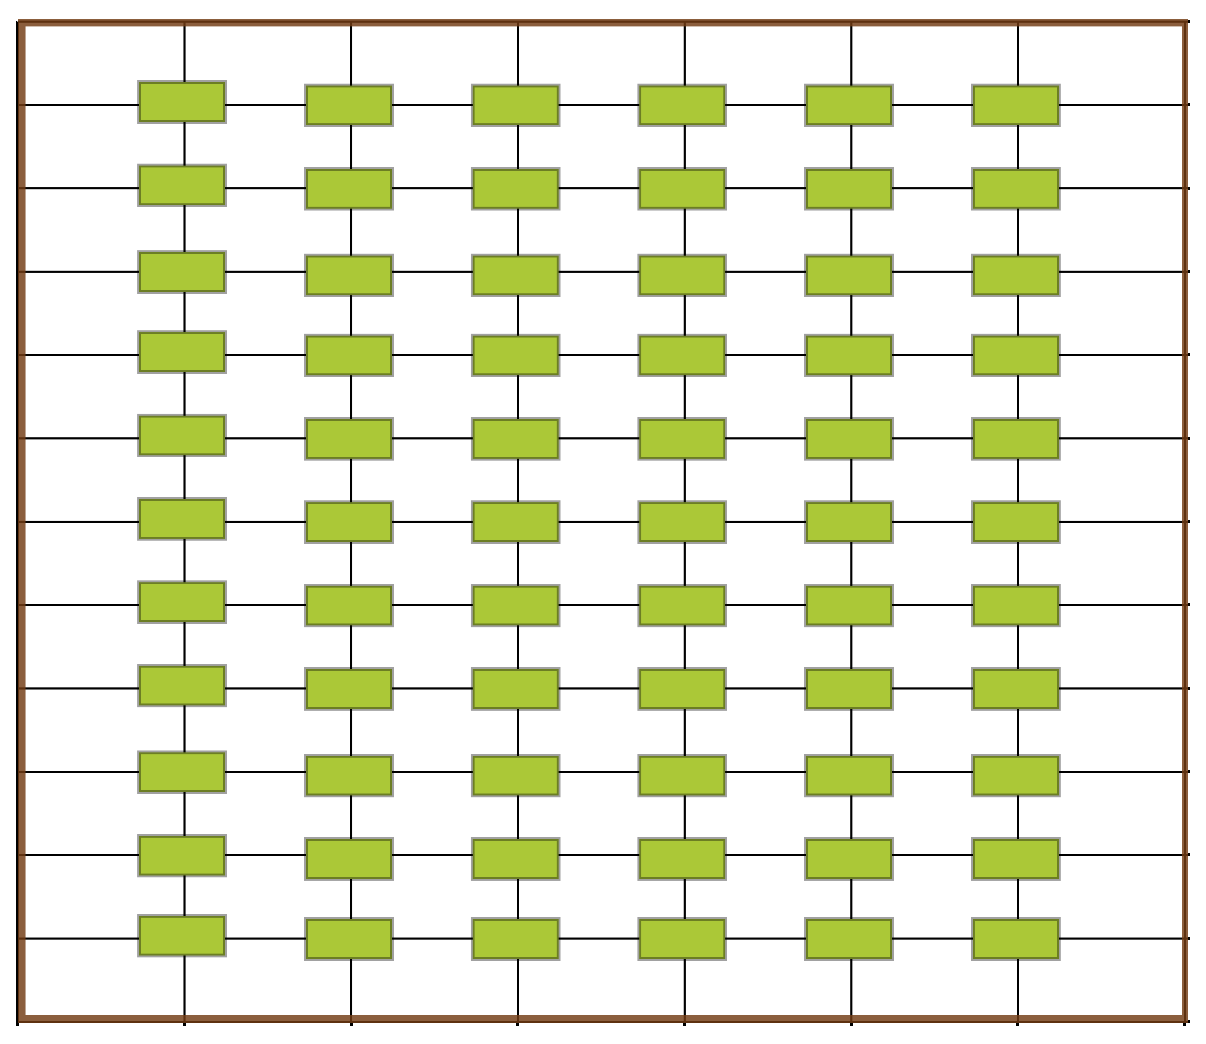
\includegraphics[width=\textwidth]{./images/fullGrid.eps}
    \end{figure}
  \end{minipage}
\end{frame}

\begin{frame}
  \frametitle{LLNL Model : Geometry}
  \begin{figure}[h!]
    \begin{center}
      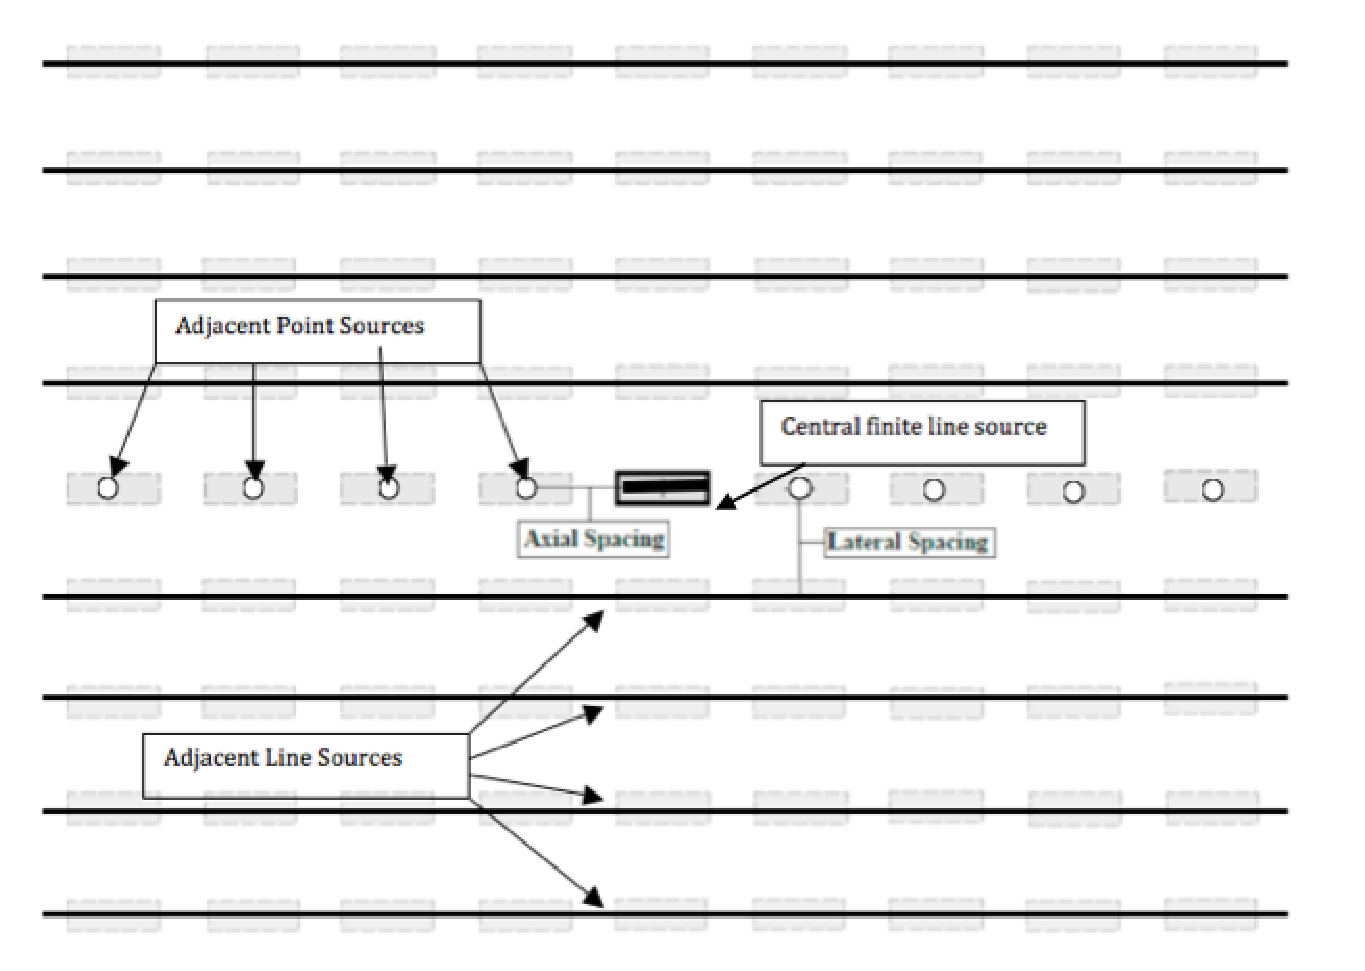
\includegraphics[width=0.7\textwidth]{./images/llnlConcept.eps}
    \end{center}
    \caption{Vertical, horizontal, alcove, and borehole emplacement layouts can 
    be represented by a line of point sources and adjacent line sources 
    \cite{sutton_investigations_2011}.}
    \label{fig:llnl}
  \end{figure}
\end{frame}

\begin{frame}
  \frametitle{LLNL Model : Solution Strategy}
  \footnotesize{
    LLNL's model is a MathCAD solution of the transient homogeneous 
    conduction equation,
    
    \begin{align}
      \nabla^2T  = \frac{1}{\alpha}\frac{\partial T}{\partial t},
      \label{condGl}
    \end{align}
    
    in which superimposed point and line source solutions approximate the repository 
    layout.
    The solution of this equation at the 
    boundary of the EBS and the waste package is then treated as a boundary condition 
    for the heterogeneous steady state equation, 
    
    \begin{align}
      \dot{q} &= U A_{out} \left( T_{in} - T_{out} \right)
      \label{condGeneral}
      \intertext{where}
      U&=\frac{1}{\sum_{i}R_i}
      \intertext{which, for the detailed EBS becomes}
      U&=\frac{1}{R_{WF}+R_{WP}+R_{buffer}+\cdots}
    \end{align}
    
    which calculates a resulting temperature gradient through the geometry at each 
    point in time for each layer surface, assuming an infinite line source 
    \cite{hardin_generic_2011, sutton_investigations_2011}. 
    }
\end{frame}



